\documentclass{article}
% --- Modify margins --- %
\usepackage{geometry}
\geometry{a4paper,scale=0.8}
% --- Involved packages --- %
\usepackage{amssymb}
\usepackage{amsthm}
\usepackage{amsmath}
\usepackage{bm}
\usepackage{graphicx}

% --- Title information --- %
\title{CS 760: Machine Learning - Fall 2020\\
        {\Large \textbf{Homework 1: Review}}\\
        {\normalsize \textbf{Due : 09/24/2020}}
    }
\author{Zijie Zhang}
\date{\today}


% --- main --- %

\begin{document}
    \maketitle
    
% --- Problem 1 ---%
\section*{Problem 1}
    \begin{proof}
        By the definition, $\mathbb{R}^D$ is a subspace if for every
        $a,\ b\in \mathbb{R}$ and every $\bm{u}, \bm{v} \in \mathbb{R}^D$,
        $a\bm{u}+b\bm{v} \in \mathbb{R}^D$.\\
        \indent It is trivial.
    \end{proof}

% --- Problem 2 ---%
\section*{Problem 2}
    \begin{proof}
        \indent
        \begin{itemize}
            \item[(a)]
                $\bm{x} = (-1,\cdots,-1) \in \mathbb{R}^D$. The element-wise square roots is
                $(i,\cdots,i) \not\in \mathbb{R}^D$.\\
                $\mathbb{R}^D$ is not closed under element-wise square roots.
            \item[(b)] 
                $\mathbb{C}^D$.
        \end{itemize}
    \end{proof}

% --- Problem 3 ---%
\section*{Problem 3}
    \begin{proof}
        For every element $\bm{x},\ \bm{y} \in \mathbb{U}$. They can be represented by a linear
        combination of $\bm{u}_1, \cdots, \bm{u}_R$.
        $$\bm{x} = \alpha_1 \bm{u}_1 + \cdots + \alpha_R \bm{u}_R$$
        $$\bm{y} = \beta_1 \bm{u}_1 + \cdots + \beta_R \bm{u}_R$$
        For every $a,\ b\in\mathbb{R}$,
        $$a\bm{x}+b\bm{y} = (a\alpha_1+b\beta_1)\bm{u}_1+\cdots+(a\alpha_R+b\beta_R)\bm{u}_R $$
        $a\bm{x}+b\bm{y} \in \mathbb{U}$, so $\mathbb{U}$ is a subspace.
    \end{proof}

% --- Problem 4 ---%
\section*{Problem 4}
    \begin{proof}
        \indent
        \begin{itemize}
            \item[(a)]
                By the \textit{Bayes rule},
                \begin{align*}
                    \mathbb{P}(&\text{Have diabetes}|\text{These genes inactive})\\
                    &= \frac{\mathbb{P}(\text{These genes inactive}|\text{Have diabetes})\cdot \mathbb{P}(\text{Have diabetes})}{\mathbb{P}(\text{These genes inactive})}
                \end{align*}
            \item[(b)]
            I need to know $\mathbb{P}(\text{These genes inactive})$.
            \item[(c)]
                If the probability that these three genes inactive is very small,
                I should be concerned.
        \end{itemize}
    \end{proof}

% --- Problem 5 ---%
\section*{Problem 5}
    \begin{proof}
        \begin{equation*}
            \mathbb{P}(x|\theta)=\left\{
                \begin{array}{rcl}
                &\theta e^{-\theta(x-t_0)} & ,{x \geqslant t_0}\\
                &0 & ,{x \leqslant t_0}
                \end{array} \right.
        \end{equation*}
        \begin{itemize}
            \item $t_0$ \textit{is the minimal time delay}:
                    $\mathbb{P}(x\leqslant t_0|\theta) = 0$
            \item \textit{Larger delays are rarer than shorter ones}:
                    For all $x,\ y\in [t_0,\infty]$, $x<y$,
                    \begin{align*}
                        \frac{\mathbb{P}(y|\theta)}{\mathbb{P}(x|\theta)}
                        &=\frac{\theta e^{-\theta(x-t_0)}}{\theta e^{-\theta(y-t_0)}}\\
                        &=e^{-\theta(x-y)}\\
                        &<1
                    \end{align*}
            \item 
        \end{itemize}
    \end{proof}

% --- Problem 6 ---%
\section*{Problem 6}
    \begin{proof}
        \indent
        \begin{itemize}
            \item[(a)]
                \begin{figure}[h!]
                    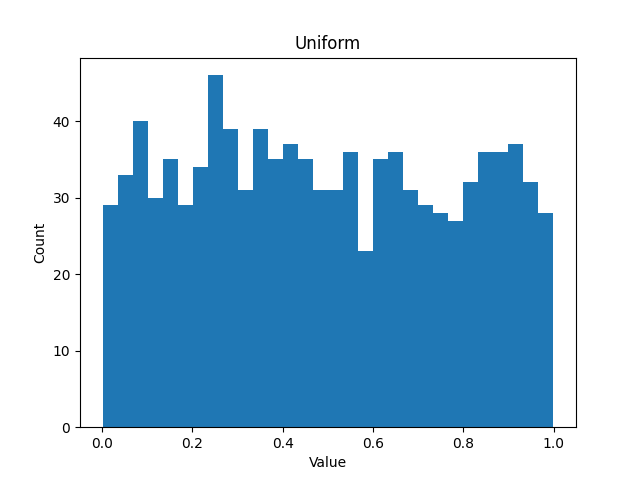
\includegraphics[height=10cm]{Q6/Figure_1.png}
                    \centering
                \end{figure}
                It doesn't look fairly uniform.
            \item[(b)] $y_i \sim \text{Bernoulli(p)}$
            \item[(c)]
                \begin{figure}[h!]
                    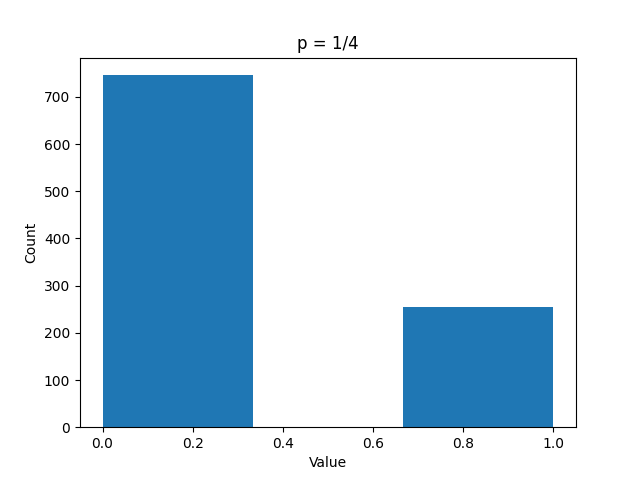
\includegraphics[width=5cm]{Q6/Figure_2.png}
                    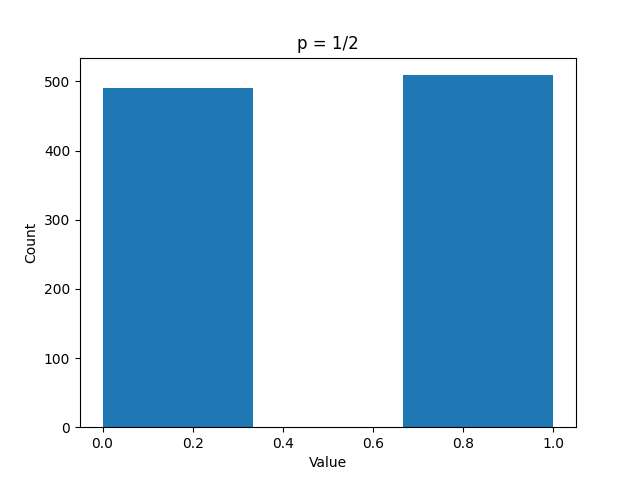
\includegraphics[width=5cm]{Q6/Figure_3.png}
                    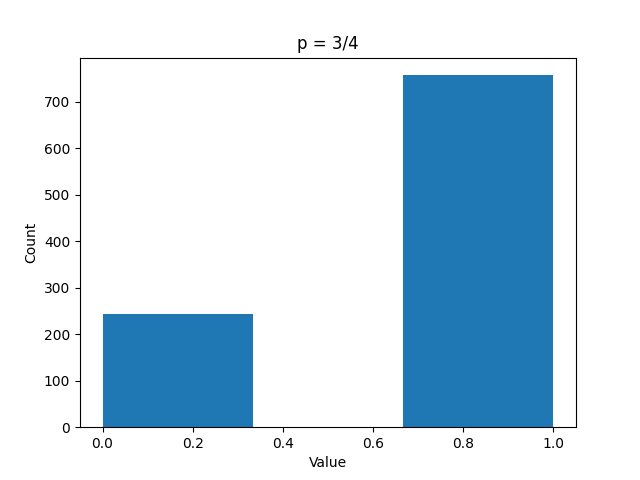
\includegraphics[width=5cm]{Q6/Figure_4.png}
                    \centering
                \end{figure}
                Yes.
            \item[(d)] $z_k \sim \text{B(n,p)}$ 
            \item[(e)]
            \begin{figure}[h!]
                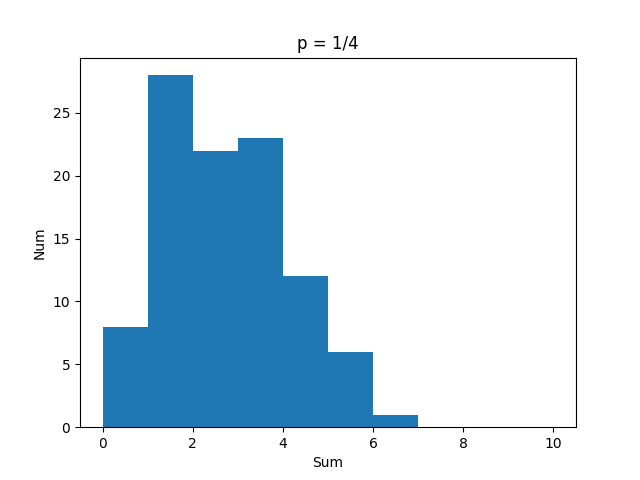
\includegraphics[width=5cm]{Q6/Figure_5.png}
                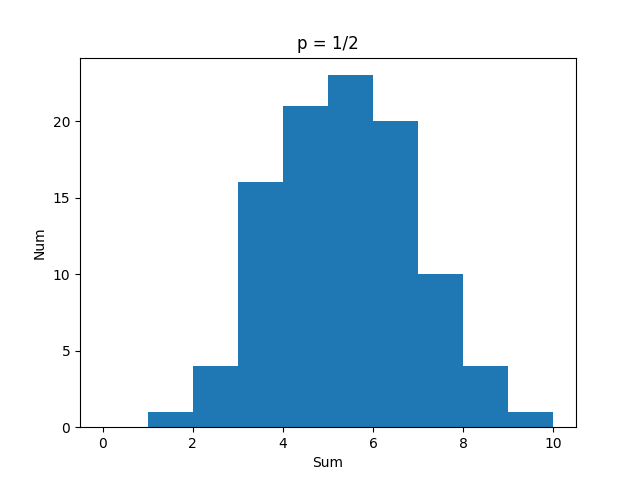
\includegraphics[width=5cm]{Q6/Figure_6.png}
                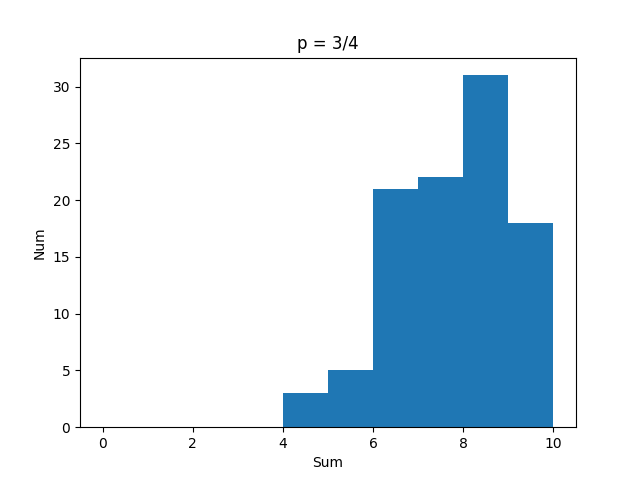
\includegraphics[width=5cm]{Q6/Figure_7.png}
                \centering
            \end{figure}
            Yes.
        \end{itemize}
    \end{proof}

% --- Problem 7 ---%
\section*{Problem 7}
    \begin{proof}
        
    \end{proof}


\end{document}